%%%%%%%%%%%%%%%%%%%%%%%%%%%%%%%%%%%%%%%%%%%%%%%%
% Corrigé UPSTI
% Concours - Epreuve - Année
%%%%%%%%%%%%%%%%%%%%%%%%%%%%%%%%%%%%%%%%%%%%%%%%
\documentclass[11pt]{article}

%%%%%%%%%%%%%%%%%%%%%%%%%%%%%%%%%%%%%%%%%%%%%%%%
% Package UPSTI_Document
%%%%%%%%%%%%%%%%%%%%%%%%%%%%%%%%%%%%%%%%%%%%%%%% 
\usepackage{UPSTI_Corrige_Concours}	% Squelette minimal
%\usepackage[UPSTI]{UPSTI_Corrige_Concours} % Chargement des packages UPSTI  (téléchargeables ici: https://www.upsti.fr/documents-pedagogiques/upsti-kit-de-demarrage-latex)

%---------------------------------%
% Packages personnalisés
%---------------------------------%
% Insérez ici les packages que vous utilisez habituellement

%%%%%%%%%%%%
% Définition des vecteurs 
%%%%%%%%%%%%
\newcommand{\vect}[1]{\overrightarrow{#1}}
\newcommand{\axe}[2]{\left(#1,\vect{#2}\right)}
\newcommand{\couple}[2]{\left(#1,\vect{#2}\right)}
\newcommand{\angl}[2]{\left(\vect{#1},\vect{#2}\right)}

\newcommand{\rep}[1]{\mathcal{R}_{#1}}
\newcommand{\quadruplet}[4]{\left(#1;#2,#3,#4 \right)}
\newcommand{\repere}[4]{\left(#1;\vect{#2},\vect{#3},\vect{#4} \right)}
\newcommand{\base}[3]{\left(\vect{#1},\vect{#2},\vect{#3} \right)}


\newcommand{\vx}[1]{\vect{x_{#1}}}
\newcommand{\vy}[1]{\vect{y_{#1}}}
\newcommand{\vz}[1]{\vect{z_{#1}}}

% d droit pour le calcul différentiel
\newcommand{\dd}{\text{d}}

\newcommand{\inertie}[2]{I\left({#1}, #2\right)}
\newcommand{\matinertie}[7]{
\begin{pmatrix}
#1 & #6 & #5 \\
#6 & #2 & #4 \\
#5 & #4 & #3 \\
\end{pmatrix}_{#7}}
%%%%%%%%%%%%
% Définition des torseurs 
%%%%%%%%%%%%

\newcommand{\ec}[2]{%
\mathcal{E}_{c\;\left(#1/#2\right)}}

\newcommand{\pext}[3]{%
\mathcal{P}_{\left(#1\rightarrow#2/#3\right)}}

\newcommand{\pint}[3]{%
\mathcal{P}_{\left(#1 \stackrel{\text{#3}}{\leftrightarrow} #2\right)}}


 \newcommand{\torseur}[1]{%
\left\{{#1}\right\}
}

\newcommand{\torseurcin}[3]{%
\left\{\mathcal{#1} \left(#2/#3 \right) \right\}
}

\newcommand{\torseurci}[2]{%
\left\{\sigma \left(#1/#2 \right) \right\}
}
\newcommand{\torseurdyn}[2]{%
\left\{\mathcal{D} \left(#1/#2 \right) \right\}
}


\newcommand{\torseurstat}[3]{%
\left\{\mathcal{#1} \left(#2\rightarrow #3 \right) \right\}
}


 \newcommand{\torseurc}[8]{%
%\left\{#1 \right\}=
\left\{
{#1}
\right\}
 = 
\left\{%
\begin{array}{cc}%
{#2} & {#5}\\%
{#3} & {#6}\\%
{#4} & {#7}\\%
\end{array}%
\right\}_{#8}%
}

 \newcommand{\torseurcol}[7]{
\left\{%
\begin{array}{cc}%
{#1} & {#4}\\%
{#2} & {#5}\\%
{#3} & {#6}\\%
\end{array}%
\right\}_{#7}%
}

 \newcommand{\torseurl}[3]{%
%\left\{\mathcal{#1}\right\}_{#2}=%
\left\{%
\begin{array}{l}%
{#1} \\%
{#2} %
\end{array}%
\right\}_{#3}%
}

% Vecteur vitesse
 \newcommand{\vectv}[3]{%
\vect{V_{{#2}/{#3}}}\left( {#1}\right)
}

% Vecteur force
\newcommand{\vectf}[2]{%
\vect{R_{ {#1} \rightarrow {#2}}}
}

% Vecteur moment stat
\newcommand{\vectm}[3]{%
\vect{\mathcal{M}_{{#2} \rightarrow {#3}}}    \left( {#1}\right)
}




% Vecteur résultante cin
\newcommand{\vectrc}[2]{%
\vect{R_{c\;{{#1}/ {#2}}}}
}
% Vecteur moment cin
\newcommand{\vectmc}[3]{%
\vect{\sigma_{{#2}/{#3}}}\left( {#1}\right)
}


% Vecteur résultante dyn
\newcommand{\vectrd}[2]{%
\vect{R_{d\;{{#1}/ {#2}}}}
}
% Vecteur moment dyn
\newcommand{\vectmd}[3]{%
\vect{\delta_{{#2}/{#3}}}\left( {#1}\right)
}

% Vecteur accélération
 \newcommand{\vectg}[3]{%
\vect{\Gamma_{{#2}/{#3}}}\left( {#1}\right)
}

% Vecteur omega
 \newcommand{\vecto}[2]{%
\vect{\Omega_{{#1}/{#2}}}
}
% }$$\left\{\mathcal{#1} \right\}_{#2} =%
% \left\{%
% \begin{array}{c}%
%  #3 \\%
%  #4 %
% \end{array}%
% \right\}_{#5}}
\usepackage{amsmath}

\usepackage{siunitx}
\sisetup{output-decimal-marker = {,}}

% ---

%---------------------------------%
% Paramètres du corrigé
%---------------------------------%

% ----------
% Concours
% ----------
% 0: Custom*
% 1: ATS
% 2: Banque PT
% 3: CCINP
% 4: CCP
% 5: CCS (par défaut)
% 6: E3A
% 7: ICNA
% 8: Mines AADN
% 9: Mines Ponts
% 10: X-ENS
% * Si on met la valeur 0, il faut décommenter la ligne suivante: 		
%\newcommand{\UPSTIconcoursCustom}{Concours custom}
\newcommand{\UPSTIidConcours}{5}

% ----------
% Filière
% ----------
% 0: Custom*
% 1: ATS
% 2: MP
% 3: MPI
% 4: PSI (par défaut)
% 5: PT
% 6: TSI
% 7: MP2I
% 8: MPSI
% 9: PCSI
% 10: PTSI
% * Si on met la valeur 0, il faut décommenter la ligne suivante: 		
%\newcommand{\UPSTIfiliereCustom}{Filière custom}
\newcommand{\UPSTIidFiliere}{4}

% ----------
% Epreuve
% ----------
% 0: Custom*
% 1: S2I (par défaut)
% 2: Informatique
% 3: Modélisation et informatique
% 4: Modélisation
% 5: Physique - SI
% 6: SI A
% 7: SI B
% 8: SI C
% 9: SI 1
% 10: SI 2
% * Si on met la valeur 0, il faut décommenter la ligne suivante: 		
%\newcommand{\UPSTIepreuveCustom}{Epreuve custom}
\newcommand{\UPSTIidEpreuve}{1}

% ----------
% Session
% ----------
\newcommand{\UPSTIsession}{2020}

% ----------
% Titre de l'épreuve (souvent, le nom du support)
% ----------
\newcommand{\UPSTItitreEpreuve}{Robotisation du désherbage mécanique des vignes}
% Si le nom est trop long pour l'entête, on peu décommenter la ligne suivante:
\newcommand{\UPSTItitreEpreuveRaccourci}{Robot Bakus}      

%----------------------------------------------- 
\UPSTIprepareDocument		% "Compile" les variables
%%%%%%%%%%%%%%%%%%%%%%%%%%%%%%%%%%%%%%%%%%%%%%%% 


%%%%%%%%%%%%%%%%%%%%%%%%%%%%%%%%%%%%%%%%%%%%%%%% 
% Début du document
%%%%%%%%%%%%%%%%%%%%%%%%%%%%%%%%%%%%%%%%%%%%%%%% 
\begin{document}
\UPSTIpreambuleEpreuve	% Affichage du préambule de l'épreuve

%---------------------------------%
% DEBUT du contenu
%---------------------------------%

%\UPSTItitrePartieCorrige{Titre de la partie}


\begin{center}
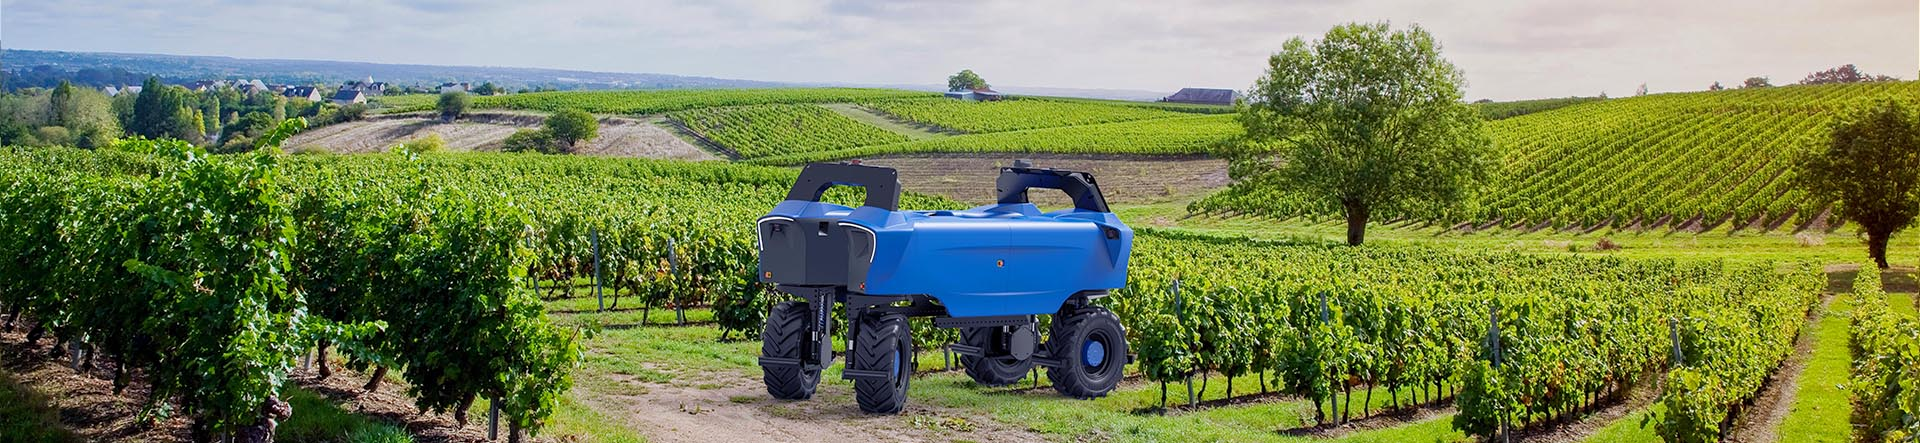
\includegraphics[width=\linewidth]{images/bakus-vigne}

\footnotesize \url{https://vitibot.fr/img/bakus-vigne.jpg}
\normalsize
\end{center}
\section{Génération des consignes d'orientation des roues avant et arrière pour le guidage du robot Bakus}

\UPSTIobjectif{
Élaborer les lois permettant de générer les consignes d'orientation à envoyer à chacune des quatre roues orientables du robot, afin qu'il puisse se déplacer le long d'un rang de vigne avec la même précision qu'un tracteur piloté par un chauffeur.
}

\subsection{Changement de variables $\left (y_{G_2},\theta \right) \rightarrow \left(y_F,y_R\right)$}

% -------------------------- 
% Boite d'objectif 
% -------------------------- 
\UPSTIobjectif{
Simplifier l'approche du problème d'asservissement du couple de variables $\left (y_{G_2},\theta \right)$ au point de fonctionnement $\left(0,0\right)$ à l'aide d'un changement de variables approprié.
}
% -------------------------- 

%\subsubsection{Test subsubsection}

% -------------------------- 
% Question (sans le saut de ligne qui la précède par défaut) + corrigé
% -------------------------- 
%\UPSTIquestion* Question (sans ligne vide, car à la suite d'un titre) On utilise la commande étoilée UPSTIquestion*

\UPSTIquestion* À partir de la figure A uniquement : 
\begin{itemize}
\item déterminer les expressions linéarisées à l'ordre 1 de $y_F$ et $y_R$, notées respectivement (E1) et (E2) en fonction de $y_{G_2}$, $\theta$ et $L$ puis en déduire l'expression de $\theta$ en fonction de $y_F$, $y_R$ et $L$ notée (E3);
\item déduire de ces résultats que chercher à asservir le couple de variables $\left (y_{G_2},\theta \right)$ au point de fonctionnement $\left(0,0\right)$  est équivalent à asservir $\left(y_F,y_R\right)$ au même point de fonctionnement.
\end{itemize}

\begin{UPSTIcorrige}

\textbf{Expression (E1)}

En se plaçant dans le quadrilatère $F F_0 G_0 G_2$, on a $\vect{F F_0} + \vect{F_0 G_0}+\vect{G_0 G_2}+\vect{G_2 F}=\vect{0}$. 

Tout d'abord, on a $\vect{G_0 F_0} = L\cos \theta \vect{x_0}$. On a alors : $y_F \vect{y_0} - L\cos \theta \vect{x_0} - y_{G_2} \vect{y_0} + L\vect{x_2}=\vect{0}$.  

On demande d'exprimer $y_F$; donc on projette cette expression suivant  $\vect{y_0}$. On obtient donc 
$y_F - y_{G_2}  + L\vect{x_2}\cdot \vect{y_0}=0$ soit $y_F - y_{G_2}  + L\sin \theta=0$ et   $y_F - y_{G_2}  + L \theta=0$  (E1).

\textbf{Expression (E2)}

En se plaçant dans le quadrilatère $G_2 G_0 R_0 R$, on a $\vect{G_2 G_0} + \vect{ G_0 R_0}+\vect{R_0 R}+\vect{R G_2 }=\vect{0}$. 

On a de même $\vect{R_0 G_0} = L\cos \theta \vect{x_0}$. On a alors : $y_{G_2} \vect{y_0} - L\cos \theta \vect{x_0} - y_{R} \vect{y_0} + L\vect{x_2}=\vect{0}$.  

On demande d'exprimer $y_R$; donc on projette cette expression suivant  $\vect{y_0}$. On obtient donc 
$y_{G_2}  - y_{R}  + L\vect{x_2}\cdot \vect{y_0}=0$ soit $y_{G_2}  - y_{R}  + L\sin \theta=0$ et $y_{G_2}  - y_{R}  + L \theta=0$ (E2).


\textbf{Expression (E3)}

On a d'une part $y_{G_2} = y_F  + L \theta$  (E1) et d'autre part $y_{G_2}  = y_{R}  - L \theta$ (E2).
En conséquence,  $y_F  + L \theta =  y_{R}  - L \theta$  soit $  \theta = \dfrac{ y_{R} - y_F}{2L } $ (E3).

\textbf{Méthode plus rapide pour déterminer (E1) et (E2)}

\begin{itemize}
\item $y_F=\vect{OF}\cdot \vect{y}_0=\left(\vect{OG_2}+\vect{G_2F}\right)\cdot \vect{y}_0$. 
On obtient alors : 
$y_F=y_{G_2}+L\vect{x}_2\cdot \vect{y}_0=y_{G_2}+L\sin\theta$ (E1).

\item $y_R=\vect{OR}\cdot \vect{y}_0=\left(\vect{OG_2}+\vect{G_2R}\right)\cdot \vect{y}_0$.
On obtient alors : 
$y_R=y_{G_2}-L\vect{x}_2\cdot \vect{y}_0=y_{G_2}-L\sin\theta$ (E2).
\end{itemize}


\textbf{Bilan}

Autour du point de fonctionnement en linéarisant les relations géométriques on obtient un système linéaire de deux équations. En effet, 
$$
\left\{
\begin{array}{l}
y_F=y_{G_2}+L\theta  \\
y_R=y_{G_2}-L\theta
\end{array}
\right.
\Rightarrow
\begin{pmatrix}
y_F \\ y_R
\end{pmatrix}
=\begin{pmatrix}
1 & -L \\ 
1 & L\\
\end{pmatrix}
\begin{pmatrix}
y_{{G_2}} \\
\theta
\end{pmatrix}.
$$

On a alors 2 relations indépendantes (E1) et (E2) pour 4 paramètres. Il y a donc deux mobilités. On peut donc choisir de piloter ou d'imposer deux couples paramètres au choix par exemple  $\left (y_{G_2},\theta \right)$ ou $\left(y_F,y_R\right)$.

Au point de fonctionnement $\left(0,0\right)$, piloter un couple de variables $\left (y_{G_2},\theta \right)$ permet de piloter de façon unique un couple $\left(y_F,y_R\right)$. Réciproquement, piloter un couple de variables $\left(y_F,y_R\right)$ permet de piloter de façon unique un couple $\left (y_{G_2},\theta \right)$.

\end{UPSTIcorrige}


\subsection{Modélisation cinématique étendue du robot}


\UPSTIobjectif{
Établir un modèle exploitable décrivant les déplacements du robot Bakus sur le sol naturel, c'est-à-dire en tenant compte d'un éventuel glissement des roues sur le sol lorsqu'il est en dévers (phénomène de dérive latérale et angulaire). 
}

\subsubsection{Notations et hypothèses}

\subsubsection{Mise en équation du modèle cinématique étendu du robot Bakus}

\UPSTIquestion* À partir de la figure A, déterminer les relations donnant les expressions de :
\begin{itemize}
\item $\dot{y}_F$ et $\dot{y_R}$ en fonction de $V_F$, $V_R$, $\theta$, $\delta_F$, $\delta_R$, $\beta_F$ et $\beta_R$;
\item $\dot{x}_{G_2}$ en fonction de $V_{G_2}$, $\gamma_{G_2}$ et $\theta$.
\end{itemize}

\begin{UPSTIcorrige}

\begin{center}
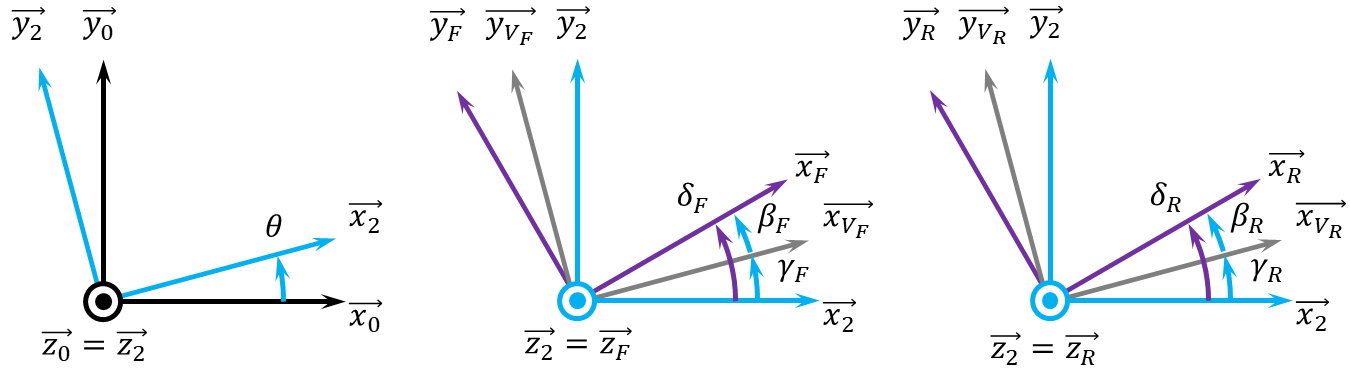
\includegraphics[width=.75\linewidth]{images/fig_01}
\end{center}
\textbf{Expression de $\dot{y}_F$}

On a  $\vectv{F}{2}{0}=\vect{V}_F = \dot{x}_F \vect{x_0} +\dot{y}_F \vect{y_0}$ (problème plan).  
Par ailleurs, en projetant $\vect{V}_F $ dans la base $\mathcal{B}_0$, on a $\vect{V}_F =V_F\vect{x_{V_F}}$ 
$=V_F\left(\cos\left(\gamma_F +\theta \right)\vect{x_0}+\sin\left(\gamma_F +\theta \right)\vect{y_0}\right)$. Enfin, $\delta_F=\gamma_F+\beta_F$ $\Leftrightarrow \gamma_F = \delta_F-\beta_F  $. 
En projetant  $\vectv{F}{2}{0}$ sur $\vect{y_0}$ on a $V_F\sin\left(\delta_F-\beta_F +\theta \right) = \dot{y}_F $.

\textbf{Autre méthode : }
$$
\dot{y}_F=\dfrac{\dd }{\dd t}\left[\vect{OF}\right]_{R_0}\cdot \vect{y}_0=\vectv{F}{2}{0}\cdot \vect{y}_0=V_F\vect{x}_VF\cdot \overrightarrow{y}_0=V_F\sin(\theta+\gamma_F)=V_F\sin(\delta_F-\beta_F+\gamma_F)
$$

\textbf{Expression de $\dot{y}_R$}

De manière analogue, on a $V_R \sin\left(\delta_R-\beta_R +\theta \right) = \dot{y}_R $.

\textbf{Expression de $\dot{x}_{G_2}$}

On a  $\vectv{G_2}{2}{0}=\vect{V}_G = \dot{x}_{G_2} \vect{x_0} +\dot{y}_{G_2} \vect{y_0}$.  
Par ailleurs, en projetant $\vect{V}_{G_2} $ dans la base $\mathcal{B}_0$, on a $\vect{V}_{G_2} =V_{G_2}\vect{x_{V_{G_2}}}$ 
$=V_{G_2}\left(\cos\left(\gamma_{G_2} +\theta \right)\vect{x_0}+\sin\left(\gamma_{G_2} +\theta \right)\vect{y_0}\right)$. 
En projetant  $\vectv{{G_2}}{2}{0}$ sur $\vect{x_0}$ on a $V_{G_2}\cos\left(\gamma_{G_2} +\theta \right) = \dot{x}_{G_2} $.


\textbf{Autre méthode : }
$$
\dot{x}_{G2}=\dfrac{\dd }{\dd t}\left[\vect{OG_2}\right]_{R_0}\cdot \vect{x}_0=\vectv{G_2}{2}{0}\cdot \vect{x}_0=V_{G_2}\vect{x}_{VG_2}\cdot \overrightarrow{x}_0=V_{G_2}\cos(\theta+\gamma_{G2})$$

\end{UPSTIcorrige}



\UPSTIquestion Montrer rigoureusement que que $\vect{V}_{G_2}\cdot\vect{x_2}$ $=\vect{V}_{F}\cdot\vect{x_2}$ $=\vect{V}_{R}\cdot\vect{x_2}$. En déduire une relation entre $V_{G_2}$, $\gamma_{G_2}$, $V_F$, $\gamma_F$, $V_R$ et $\gamma_R$. 

\begin{UPSTIcorrige}

Le châssis 2 est considéré comme un solide indéformable. Le champ des vitesses de 2/0 est donc un champ de vitesse équiprojectif.
On a donc $\vect{V_{G_2}}\cdot\vect{x_2} =  \vect{V_{F}}\cdot\vect{x_2}  = \vect{V_{R}}\cdot\vect{x_2} $.
En conséquences, 
$V_{G_2} \vect{x_{V_{G_2}}} \cdot \vect{x_2} 
=V_{F} \vect{x_{V_{F}}} \cdot \vect{x_2} 
=V_{R} \vect{x_{V_{R}}} \cdot \vect{x_2} $
$\Rightarrow V_{G_2} \cos \gamma_{G_2} = V_{F} \cos \gamma_{F} =V_{R} \cos\gamma_R $.


\vspace{1cm}

{\footnotesize S'il s'agissait de remontrer les propriétés d'équiprojectivité du champ des vitesses, on peut procéder comme suit.

\begin{itemize}
\item \textbf{Soit en passant par le point $I_{20}$ :}

On a $\vect{V}_{G_2} \cdot \vect{x_2}=\left(\vect{V}_{I_{20}}+\vect{G_2 I_{20}}\wedge \vecto{2}{0}\right)  \cdot \vect{x_2}$. $\vect{V}_{I_{20}}=\vect{0}$; donc $\vect{V}_{G_2} \cdot \vect{x_2}=\left(\left(\rho \vect{y_2} - \left(h+L\right)\vect{x_2}\right) \wedge \vecto{2}{0}\right)  \cdot \vect{x_2}$ .  $\left(\vect{x_2}\wedge \vect{u}\right)\cdot \vect{x_2} = 0$; donc 
$\vect{V}_{G_2} \cdot \vect{x_2}=\left(\rho \vect{y_2}  \wedge  \dot{\theta} \vect{z_2}\right)  \cdot \vect{x_2}$
$=\rho \dot{\theta} $.

De même,  $\vect{V}_{F} \cdot \vect{x_2} =\left(\vect{V}_{I_{20}}+\vect{F I_{20}}\wedge \vecto{2}{0}\right) \cdot \vect{x_2}$
$=\left(\left(\rho \vect{y_2} - \left(h+2L\right)\vect{x_2}\right)\wedge \vecto{2}{0}\right) \cdot \vect{x_2}$
$=\left(\rho \vect{y_2} \wedge  \dot{\theta} \vect{z_2}\right) \cdot \vect{x_2}$
$=\rho \dot{\theta} $.

Enfin, $\vect{V}_{R}\cdot \vect{x_2}=\left(\vect{V}_{I_{20}}+\vect{R I_{20}}\wedge \vecto{2}{0}\right) \cdot \vect{x_2}$
$=\left( \left(\rho \vect{y_2} - h\vect{x_2}\right)\wedge \vecto{2}{0}\right) \cdot \vect{x_2}$
$=\left(\rho \vect{y_2} \wedge \dot{\theta} \vect{z_2}\right) \cdot \vect{x_2}$
$=\rho \dot{\theta} $.

On a donc $\vect{V}_{G_2}\cdot\vect{x_2}$ $=\vect{V}_{F}\cdot\vect{x_2}=\vect{V}_{R}\cdot\vect{x_2} = \rho\dot{\theta}$.

\item \textbf{Soit en passant par les trois points $G_2$, $F$ et $R$ :}

$\vect{V}_{G_2}\cdot\vect{x_2} $ $=\vectv{G_2}{2}{0}\cdot \vect{x}_2$ $=\left(\vectv{F}{2}{0}+\vect{G_2F}\wedge \dot{\theta}\vect{z}_{0,2}\right)\cdot \vect{x}_2$ $=\vect{V}_{F}\cdot\vect{x_2}+\left(L\vect{x}_2\wedge \dot{\theta}\vect{z}_{0,2}\right)\cdot \vect{x}_2$ et $\vect{V}_{G_2}\cdot\vect{x_2}=\vect{V}_{F}\cdot\vect{x_2}$.

De même entre $G_2$ et $R$ : 
$\vect{V}_{G_2}\cdot\vect{x_2}$  $=\vectv{G_2}{2}{0}\cdot \vect{x}_2$ $=\left(\vectv{R}{2}{0}+\vect{G_2R}\wedge \dot{\theta}\vect{z}_{0,2}\right)\cdot \vect{x}_2$ $=\vect{V}_{R}\cdot\vect{x_2}+\left(-L\vect{x}_2\wedge \dot{\theta}\vect{z}_{0,2}\right)\cdot \vect{x}_2$ et $\vect{V}_{G_2}\cdot\vect{x_2}=\vect{V}_{R}\cdot\vect{x_2}$.

\end{itemize}

Par ailleurs : 
\begin{itemize}
\item $\vect{V}_{G_2}\cdot\vect{x_2} = V_{G_2} \vect{x_{V_{G_2}}} \cdot\vect{x_2}$ $=V_{G_2} \cos \gamma_{G_2}$;
\item $\vect{V}_{F}\cdot\vect{x_2}={V}_{F}\vect{x_{V_F}}\cdot\vect{x_2}$  $=V_{F} \cos \gamma_{F}$;
\item $\vect{V}_{R}\cdot\vect{x_2}={V}_{R}\vect{x_{V_R}}\cdot\vect{x_2}$   $=V_{R} \cos \gamma_{R}$.
\end{itemize}

On a donc  $V_{G_2} \cos \gamma_{G_2}=V_{F} \cos \gamma_{F}=V_{R} \cos \gamma_{R}$.
}

\normalsize

\end{UPSTIcorrige}



\UPSTIquestion À partir du résultat obtenu à la question 3, donner les expressions de $V_F$ et $V_R$ en fonction de $V_{G_2}$, $\delta_F$, $\beta_F$, $\delta_R$ et $\beta_R$. 

\begin{UPSTIcorrige}
%\textbf{TODO A FINIR !!}

On a $V_{F}  =V_{G_2} \dfrac{\cos \gamma_{G_2}}{\cos \gamma_{F}}$ 
$=V_{G_2} \dfrac{\cos \gamma_{G_2}}{\cos  \left(\delta_F-\beta_F \right)}$. 

%Or, $\tan \gamma_{G_2} = \dfrac{\tan \gamma_F+\tan \gamma_R}{2}$. 
%D'où
%$V_{F}  =V_{G_2} \dfrac{\cos \left(\arctan \left( \dfrac{\tan \gamma_F+\tan \gamma_R}{2}\right) \right) }{\cos  \left(\delta_F-\beta_F \right)}$.  
%De plus $I_{20}G_2 = \sqrt{\left(h+L\right)^2+\rho^2}$.

De même, $V_{R}  =V_{G_2} \dfrac{\cos \gamma_{G_2}}{\cos \gamma_{R}}$ $=V_{G_2} \dfrac{\cos \gamma_{G_2}}{\cos  \left(\delta_R-\beta_R \right)}$.


Or, $\tan \gamma_{G_2} = \dfrac{\tan \gamma_F+\tan \gamma_R}{2}$ soit $ \gamma_{G_2} = \arctan\left(\dfrac{\tan \gamma_F+\tan \gamma_R}{2}\right)$ $= \arctan\left(\dfrac{\tan \left(\delta_F - \beta_F\right)+\tan \left(\delta_R - \beta_R\right)}{2}\right)$. 

On injecte alors cette expression dans $V_{F}$ et $V_R$ :

$$
V_F = V_{G_2} \dfrac{\cos \left( \arctan\left(\dfrac{\tan \left(\delta_F - \beta_F\right)+\tan \left(\delta_R - \beta_R\right)}{2}\right)\right)}{\cos  \left(\delta_F-\beta_F \right)} 
$$
$$
V_R = V_{G_2} \dfrac{\cos \left( \arctan\left(\dfrac{\tan \left(\delta_F - \beta_F\right)+\tan \left(\delta_R - \beta_R\right)}{2}\right)\right)}{\cos  \left(\delta_R-\beta_R \right)} 
$$

\textbf{Est-ce vraiment la solution attendue ?}

\end{UPSTIcorrige}


\subsection{Mesure en estimation des variables du modèle cinématique étendu}

\UPSTIobjectif{ Donner les moyens au robot de mesurer ou, à défaut, d'estimer les valeurs des variables $\delta_F$, $\delta_R$, $y_{G_2}$, $\theta$, $\dot{y}_F$ et $\dot{y}_R$ et $V_{G_2}$ du modèle cinématique étendu.
}

\subsubsection{Variables mesurées directement par des capteurs dédiés}

\UPSTIquestion Compte-tenu du contexte d’utilisation du robot, justifier l’intérêt d’avoir choisi des codeurs absolus
plutôt que relatifs (incrémentaux) pour obtenir les valeurs mesurées de $\delta_F$ et $\delta_R$.

\begin{UPSTIcorrige}

Ne connaissant pas la technologie du codeur absolu, on ne voit pas clairement l'intérêt de choix par rapport à un codeur incrémental. Un critère de choix pourrait aussi être la résolution du codeur vis-à-vis de la précision attendue sur la position angulaire.

On pourrait aussi justifier le choix par la connaissance de l'angle à la mise à l'énergie qui ne nécessite pas de faire une initialisation avec un codeur absolu.  
\end{UPSTIcorrige}

\subsubsection{Variables estimées par analyse d’images des huit caméras TOF du robot}

\UPSTIquestion À partir des équations (I.2) et (I.3), donner l’expression des variables estimées $\hat{\beta}_F$
et $\hat{\beta}_R$ en fonction des variables mesurées $\dot{y}_F$, $\dot{y}_R$, $V_{G_2}$, $\theta$, $\delta_F$ et $\delta_R$.

\begin{UPSTIcorrige}
On a $\dot{y}_F =V_{G_2} \left(\theta + \delta_F - \beta_F\right)$ et $\dot{y}_R =V_{G_2} \left(\theta + \delta_R - \beta_R\right)$. Par conséquent, $\hat{\beta}_F =\theta + \delta_F-\dfrac{\dot{y}_F}{V_{G_2} }  $ et $\hat{\beta}_R =\theta + \delta_R-\dfrac{\dot{y}_R}{V_{G_2} }  $.
\end{UPSTIcorrige}



\subsection{Génération des consignes d’orientation des roues $\left(\delta^*_F,\delta^*_R\right)$ pour l’asservissement latéral et angulaire du robot enjambeur le long d’un rang de vigne}
\UPSTIobjectif{ 
Établir les lois de génération de consigne de l’asservissement latéral du robot Bakus pour qu’il puisse
suivre avec précision la trajectoire $\mathcal{T}$, malgré un glissement éventuel des roues sur le sol naturel
}

\subsubsection{Passage du domaine temporel au domaine spatial : $t\to x_{G_2}$}
\UPSTIobjectif{ 
Rendre le modèle cinématique étendu indépendant de la vitesse linéaire $V_{G_2}$
du robot le long d’un rang de vigne, afin de découpler la gestion des écarts latéraux $y_F$ et $y_R$ et celui de la vitesse d’avance $V_{G_2}$.}



%%%%%%%%%%%%%%%%%%%%%%%%%%%%%%%%%


\UPSTIquestion À partir des équations (E3), (I.1), (I.2) et (I.3) établies à partir du modèle cinématique étendu de la
figure A, montrer que : 
$$ \begin{array}{lr}
y'_F = \theta + \delta_F-\beta_F   & \text{(I.4)} \\
y'_R = \theta + \delta_R-\beta_R  & \text{(I.5)}\\
\theta'=\dfrac{y'_F-y'_R}{2L}       & \text{(I.6)}
\end{array}.$$

\begin{UPSTIcorrige}


On a les résultats suivants :  $  \theta = \dfrac{ y_{R} - y_F}{2L }$ (E3), d'après  (I.1), (I.2) et (I.3), $\dot{x}_{G_2}=V_{G_2}$, $\dot{y_F}=V_{G_2}\left(\theta + \delta_F - \beta_F\right)$ et  $\dot{y_R}=V_{G_2}\left(\theta + \delta_R - \beta_R\right)$. 


D'après (I.1), $\dot{x}_{G_2}= \dfrac{\dd x_{G_2}}{\dd t} =  V_{G_2}$.
Par ailleurs (\textbf{à confirmer}) on cherche $y'_F=\dfrac{\dd y_F}{\dd x_{G_2}} $ 
$= \dfrac{\dd y_F}{\dd t}  \cdot \dfrac{\dd  t}{\dd x_{G_2}}$ 
$ =\dot{y_F}\cdot \dfrac{1}{V_{G_2}}$ 
$ =\theta + \delta_F - \beta_F$.

On montre de même que $y'_R = \theta + \delta_R-\beta_R$

Enfin, $\theta' = \dfrac{\dd \theta}{\dd x_{G_2}}=\dfrac{ \dfrac{\dd y_{R}}{\dd x_{G_2}} - \dfrac{\dd y_F}{\dd x_{G_2}}}{2L } = \dfrac{y'_R-y'_F}{2L}$.

\textbf{Attention : le sujet propose l'opposé de ce résultat.}

\end{UPSTIcorrige}

\subsubsection{Asservissement de la variable de déplacement latéral $y_F$ à une consigne $y^*_F=0$}

\UPSTIobjectif{Justifier le choix du modèle du comportement en déplacement latéral $y_F$ du robot assurant sa convergence à une valeur de consigne $y_F^*$ et son réglage}

\UPSTIquestion Par analogie avec un modèle temporel usuel d’ordre 2 à identifier, de paramètres caractéristiques $\omega_{0F}$, $\xi_F$ et $K_F$ :
\begin{itemize}
\item en justifiant la réponse, tracer l’allure de l’évolution de  $y_F\left(x_{G_2}\right)$  imposée par le modèle 1 (I.7) pour une consigne $y_F^*=0$ en fonction de $x_{G_2}$, lorsque $y_F\left(x_{G_2}=0\right)=y_{F0}>0$
 ($y_{F0}$ étant une valeur constante), $y'_F\left(x_{G_2}=0\right)=0$, $K_{pF}=\dfrac{K^2_{dF}}{4}$ et $K_{dF}\simeq 5$; 
 \item préciser sur le graphe les éléments caractéristiques de la courbe tracée pour $x_{G_2}=0$ ;
\item justifier pourquoi le paramètre $K_{pF}$ a été réglé de telle sorte que $K_{pF}=\dfrac{K^2_{dF}}{4}$, compte-tenu du contexte de fonctionnement du robot enjambeur.
\end{itemize}

\begin{UPSTIcorrige}

\textbf{Identification des  caractéristiques $\omega_{0F}$, $\xi_F$ et $K_F$}

En utilisant l'analogie avec un modèle temporel, on a $s'' + 2\xi_F\omega_{0F} s' + \omega_{0F}^2 s = K_Fe\omega_0^2$ à identifier avec la relation $y''_F+K_{dF}y'_F+K_{pF}y_F=K_{pF}y^*_F$.
On a alors  $\omega_{0F}^2 =K_{pF}$, $K_{pF} = K_F\omega_{0F}^2$ soit $K_F=1$. De plus, $2\xi_F\omega_{0F} = K_{dF}$ soit $\xi_F = \dfrac{K_{dF}}{2\omega_{0F}}= \dfrac{K_{dF}}{2\sqrt{K_{pF}}}$.

On a donc $\omega_{0F}=\sqrt{K_{pF}}$, $\xi_F=\dfrac{K_{dF}}{2\sqrt{K_{pF}}} $ et $K_F=1$.


\textbf{Tracer de l’allure de l’évolution de  $y_F\left(x_{G_2}\right)$}
En utilisant les valeurs proposées, $\xi_F=\dfrac{K_{dF}}{2\sqrt{K_{pF}}}\dfrac{K_{dF}}{2\dfrac{K_{dF}}{2}} =1 $ et $\omega_{0F}=\sqrt{\dfrac{5^2}{4}}=\dfrac{5}{2}$. L'allure de l'évolution de $y_F\left(x_{G_2}\right)$ est donc celle d'un second ordre amorti. Il y a donc une tangente horizontale à l'origine (ce qui est confirmé par le fait qu'il soit indiqué que $y'_F\left(x_{G_2}=0\right)=0$.

\begin{center}
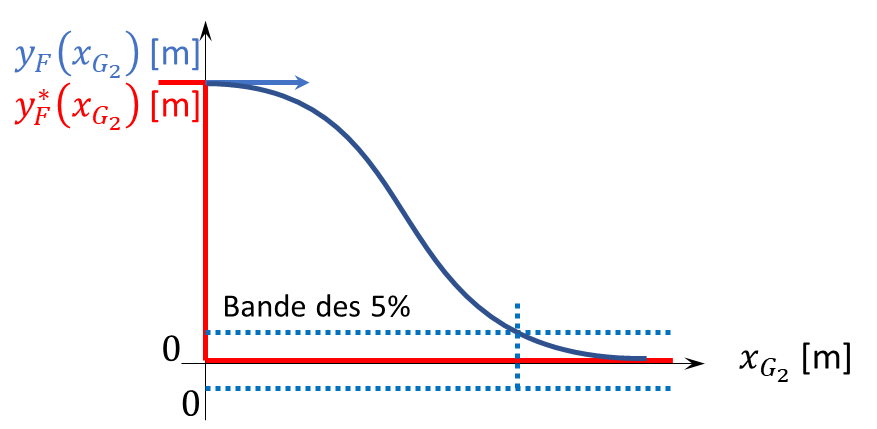
\includegraphics[width=.6\linewidth]{images/fig_05_bis}
\end{center}
\textbf{Justifier que $K_{pF}=\dfrac{K^2_{dF}}{4}$}
En ayant fait ce choix pour $K_{pF}$, on assure un $\xi=1$ donc un système le plus rapide possible sans dépassement. 
Cela permet d'éviter les oscillations autour de la trajectoire cible et donc de limiter les problèmes de glissement. 

\end{UPSTIcorrige}


\UPSTIquestion Expliquer ce que représente $x_{F_{r5\%}}$ dans le cas de ce modèle spatial (I.8), analogue du temps de réponse à \SI{5}{\%} dans le cas d’un modèle temporel. Préciser son unité. Compte-tenu de la valeur prise précédemment pour le réglage de $K_{pF}$, donner alors une expression littérale approchée de  $x_{F_{r5\%}}$ en fonction de $K_{dF}$. Effectuer
l’application numérique et conclure sur la pertinence de la valeur numérique de $K_{dF}$, vu le contexte d’utilisation
du robot enjambeur.

\begin{UPSTIcorrige}
$x_{F_{r5\%}}$ représente la distance que met le robot à être à une distance inférieure à \SI{5}{\%} de la trajectoire. Elle s'exprime en mètres (si toutes les distance sont en mètres).

D'après l'abaque du temps de réponse à \SI{5}{\%} pour un système d'ordre 2, on a  $\omega_{0F} x_{F_{r5\%}}\simeq 5$ pour $\xi_F=1$  \textbf{(ce résultat ne me semble pas exigible dans le programme de PCSI-PSI)}. On a alors 
$x_{F_{r5\%}} \simeq \dfrac{5}{\omega_{0F} }$ $\simeq\dfrac{5}{\sqrt{K_{pF}}}$ $\simeq \dfrac{5\times 2}{K_{dF}}$ $\simeq \SI{2}{m}$.
Cela semble réaliste compte-tenu de la longueur des rangs de vignes.
\end{UPSTIcorrige}

\subsubsection{Génération des consignes d'orientation $\delta_F^*$ et $\delta_R^*$ des roues médianes}
\UPSTIobjectif{ Établir deux relations permettant de déterminer la consigne d’orientation de la roue médiane avant
$\delta_F^*$ et celle de la roue médiane arrière $\delta_R^*$ (figure A).}


\UPSTIquestion À partir des relations issues du modèle cinématique étendu du robot (figure A), de la relation issue
du modèle 1 choisi pour le comportement de $y_F\left(x_{G_2}\right)$, et en sachant que les relations (E1) et (E2) trouvées à la question 1 permettent de considérer que les valeurs des variables $y_F$ et $y_F$ sont connues si $y_{G_2}$ et $\theta$ le sont aussi (trajectoire $\mathcal{T}$ connue) :
\begin{enumerate}
\item déterminer l’expression de $y''_F$, en fonction de $\delta_F$, $\beta_F$, $\delta_R$, $\beta_R$ et $L$. Pour ce faire, commencer par exprimer $y''_F$ à partir de la relation (I.4), en tenant compte de l’hypothèse relative aux valeurs de $\delta'_F-\beta'_F$;
\item en tenant compte du point de fonctionnement souhaité, déterminer ensuite l’expression de $\delta_F$ de la roue
médiane avant 5, en utilisant la relation (I.7), puis les relations (I.4) et (E3) ;
\item en identifiant précisément les variables qui sont mesurées et estimées, et en supposant que les dispositifs
d’orientation des roues fonctionnent parfaitement et assurent ainsi que $\delta^*_F = \delta_F$, montrer alors que l’expression de $\delta^*_F$ est de la forme $\delta^*_F =C_1 \hat{\beta}_F +C_2\left(\delta_R - \hat{\beta}_R\right)+C_3 y_F + C_4 y_R$;
\item donner les expressions littérales de $C_1$, $C_2$, $C_3$ et $C_4$ en fonction de $K_{dF}$, $K_{pF}$ et $L$.
\end{enumerate}

%%%%%%%%%%%%%%%%%%%%%%
%%%%%%%%% A VOIR %%%%%%%%%
%%%%%%%%%%%%%%%%%%%%%%

 
 

\begin{UPSTIcorrige}
\textbf{Déterminer l’expression de $y''_F$, en fonction de $\delta_F$, $\beta_F$, $\delta_R$, $\beta_R$ et $L$}


D'après la relation (I.4), on a : $y'_F = \theta + \delta_F-\beta_F$. On  alors $y''_F =\dfrac{\dd y'_F}{\dd x_{G_2}} = \theta' + \delta_F'-\beta_F'$.
 En utilisant l'hypothèse $\delta_F'-\beta_F' \simeq 0$, on a alors  $y''_F =\theta'$ et donc $y''_F =  \dfrac{y'_F-y'_R}{2L}$ (I.6). On utilise alors (I.4) et (I.5) et donc $y''_F =  \dfrac{\theta +\delta_F - \beta_F  - \theta -\delta_R + \beta_R }{2L}$ $=\dfrac{\delta_F - \beta_F   -\delta_R + \beta_R }{2L}$.

\textbf{En prenant compte du résultat de la question 7, on  a $y''_F =\dfrac{-\delta_F + \beta_F   +\delta_R - \beta_R }{2L}$. C'est cette expression que nous conserverons pour la suite.}


%D'après la relation (I.4), on a : $y'_F = \theta + \delta_F-\beta_F$. On  alors $y''_F =\dfrac{\dd y'_F}{\dd x_{G_2}} = \theta' + \delta_F'-\beta_F'$. Or en utilisant (I.6), on obtient 
%$y''_F = \dfrac{y'_F-y'_R}{2L} + \delta_F'-\beta_F'$. En utilisant a nouveau (I.4) et (I.5), 
%$y''_F = \dfrac{\left(\theta + \delta_F-\beta_F\right)-\left(\theta + \delta_R-\beta_R\right)}{2L} + \delta_F'-\beta_F'$
%soit $y''_F = \dfrac{ \delta_F- \delta_R +\beta_R-\beta_F}{2L} + \delta_F'-\beta_F'$.
%
%En tenant compte de l'hypothèse du sujet, $ \delta_F'-\beta_F'\simeq 0$ et 
%$y''_F = \dfrac{ \delta_F- \delta_R +\beta_R-\beta_F}{2L}$.

\textbf{Déterminer ensuite l’expression de $\delta_F$}

D'après (I.7), on a $y''_F  + K_{dF}y'_F+K_{pF}y_F = K_{pF}y_F^*$. En utilisant (I.4),  
$y''_F  + K_{dF}\left(  \theta + \delta_F-\beta_F \right)+K_{pF}y_F = K_{pF}y_F^*$.
Enfin en utilisant (E3), 
$y''_F  + K_{dF}\left(  \dfrac{y_R-y_F}{2L} + \delta_F-\beta_F \right)+K_{pF}y_F = K_{pF}y_F^*$.

On a donc 
$K_{dF} \delta_F  = K_{pF}y_F^* - y''_F - K_{pF}y_F- K_{dF}\left(  \dfrac{y_R-y_F}{2L} -\beta_F \right)$

$\Leftrightarrow  \delta_F  = \dfrac{K_{pF}}{K_{dF}}y_F^* - \dfrac{y''_F}{K_{dF}} - \dfrac{K_{pF}}{K_{dF}}y_F- \left(  \dfrac{y_R-y_F}{2L} -\beta_F \right)$.

\textbf{Montrer que $\delta^*_F =C_1 \hat{\beta}_F +C_2\left(\delta_R - \hat{\beta}_R\right)+C_3 y_F + C_4 y_R$}

En utilisant les relations précédentes, on a 
%$\delta_F  = \dfrac{K_{pF}}{K_{dF}}y_F^* - \dfrac{1}{K_{dF}}\left(  \dfrac{ \delta_F- \delta_R +\beta_R-\beta_F}{2L} \right) - \dfrac{K_{pF}}{K_{dF}}y_F- \left(  \dfrac{y_R-y_F}{2L} -\beta_F \right)$.
$\delta_F  = \dfrac{K_{pF}}{K_{dF}}y_F^* - \dfrac{1}{K_{dF}}\left(  \dfrac{ -\delta_F+ \delta_R -\beta_R+\beta_F}{2L} \right) - \dfrac{K_{pF}}{K_{dF}}y_F- \left(  \dfrac{y_R-y_F}{2L} -\beta_F \right)$.


On peut montrer que  $\hat{\beta}_F= {\beta}_F$ et $\hat{\beta}_R= {\beta}_R$.

(En effet : $\hat{\beta}_F = \theta + \delta_F -\dfrac{\dot{y}_F}{V_{G_2}}$ 
$=\dfrac{y_R-y_F}{2L}+ \delta_F -\dfrac{\dot{y}_F}{V_{G_2}}$
$=\dfrac{y_R-y_F}{2L}+ \delta_F -\dfrac{V_{G_2}\left( \theta+\delta_F-\beta_F\right)}{V_{G_2}}$
$=\dfrac{y_R-y_F}{2L} -\left( \dfrac{y_R-y_F}{2L}-\beta_F\right)$ $=\beta_F$).


On a donc 
%$\delta_F  = \dfrac{K_{pF}}{K_{dF}}y_F^* - \dfrac{1}{K_{dF}}\left(  \dfrac{ \delta_F- \delta_R +\hat{\beta}_R-\hat{\beta}_F}{2L} \right) - \dfrac{K_{pF}}{K_{dF}}y_F-   \dfrac{y_R-y_F}{2L} +\hat{\beta}_F $
$\delta_F  = \dfrac{K_{pF}}{K_{dF}}y_F^* - \dfrac{1}{K_{dF}}\left(  \dfrac{ -\delta_F+ \delta_R -\hat{\beta}_R+\hat{\beta}_F}{2L} \right) - \dfrac{K_{pF}}{K_{dF}}y_F-   \dfrac{y_R-y_F}{2L} +\hat{\beta}_F $


$\Leftrightarrow \delta_F  = \dfrac{K_{pF}}{K_{dF}}y_F^* - \dfrac{1}{2L K_{dF}}\left(  - \delta_F+ \delta_R -\hat{\beta}_R+\hat{\beta}_F \right) - \dfrac{K_{pF}}{K_{dF}}y_F   -   \dfrac{y_R}{2L}+   \dfrac{y_F}{2L} +\hat{\beta}_F $



$\Leftrightarrow \delta_F  = \dfrac{K_{pF}}{K_{dF}}y_F^* 
+\dfrac{ \delta_F}{2L K_{dF}}
%+\dfrac{1}{2L K_{dF}}\left(  \hat{\beta}_F \right)  
+  \left(1-\dfrac{1}{2L K_{dF}}\right)\hat{\beta}_F
+\dfrac{1}{2L K_{dF}}\left(   -\delta_R +\hat{\beta}_R \right)  
+\left( \dfrac{1}{2L}  - \dfrac{K_{pF}}{K_{dF}}\right)y_F 
- \dfrac{y_R}{2L} $

$\Leftrightarrow \delta_F  \left(1- \dfrac{ 1}{2L K_{dF}}\right)= \dfrac{K_{pF}}{K_{dF}}y_F^* 
%+\dfrac{1}{2L K_{dF}}\left(  \hat{\beta}_F \right)  
+  \left(1-\dfrac{1}{2L K_{dF}}\right)\hat{\beta}_F
+\dfrac{1}{2L K_{dF}}\left(  - \delta_R +\hat{\beta}_R \right)  
+\left( \dfrac{1}{2L}  - \dfrac{K_{pF}}{K_{dF}}\right)y_F 
- \dfrac{y_R}{2L} $


$\Leftrightarrow \delta_F  = \dfrac{2L K_{pF}}{ 2L K_{dF}-1}y_F^* 
%+\dfrac{1}{2L K_{dF}}\left(  \hat{\beta}_F \right)  
+ \hat{\beta}_F
+\dfrac{1}{ 2L K_{dF}-1}\left(  - \delta_R +\hat{\beta}_R \right)  
+ \dfrac{K_{dF}- 2L K_{pF}}{ 2L K_{dF}-1}y_F 
- \dfrac{ K_{dF}}{ 2L K_{dF}-1} {y_R}$

$\Leftrightarrow \delta_F  = 
\hat{\beta}_F
+\dfrac{1}{1- 2L K_{dF}}\left(  \delta_R -\hat{\beta}_R \right)  
+ \dfrac{K_{dF}- 2L K_{pF}}{ 2L K_{dF}-1}y_F 
+ \dfrac{ K_{dF}}{1- 2L K_{dF}} {y_R}
+\dfrac{2L K_{pF}}{ 2L K_{dF}-1}y_F^* $
%+\dfrac{1}{2L K_{dF}}\left(  \hat{\beta}_F \right)  


%$\Leftrightarrow \delta_F   \dfrac{ 1+2L K_{dF}}{2L K_{dF}}= 
%$\Leftrightarrow \delta_F   = 
%\dfrac{2L K_{pF}}{ -1+2L K_{dF}}  y_F^* 
%+\hat{\beta}_F
%+\dfrac{1}{ 1-2L K_{dF}} \left( \delta_R -\hat{\beta}_R \right)  
%+\dfrac{K_{dF} - 2LK_{pF}}{ -1+2L K_{dF}} y_F 
%- \dfrac{ K_{dF}}{ -1+2L K_{dF}}y_R $.




%$\Leftrightarrow \delta_F  = \dfrac{K_{pF}}{K_{dF}}y_F^* - \dfrac{1}{2L K_{dF}}\left(   \delta_F- \delta_R +\hat{\beta}_R-\hat{\beta}_F \right) - \dfrac{K_{pF}}{K_{dF}}y_F   -   \dfrac{y_R}{2L}+   \dfrac{y_F}{2L} +\hat{\beta}_F $
%
%$\Leftrightarrow \delta_F  = \dfrac{K_{pF}}{K_{dF}}y_F^* 
%-\dfrac{ \delta_F}{2L K_{dF}}
%%+\dfrac{1}{2L K_{dF}}\left(  \hat{\beta}_F \right)  
%+  \left(1+\dfrac{1}{2L K_{dF}}\right)\hat{\beta}_F
%+\dfrac{1}{2L K_{dF}}\left(   \delta_R -\hat{\beta}_R \right)  
%+\left( \dfrac{1}{2L}  - \dfrac{K_{pF}}{K_{dF}}\right)y_F 
%- \dfrac{y_R}{2L} $
%
%$\Leftrightarrow \delta_F  \left(1+ \dfrac{ 1}{2L K_{dF}}\right)= \dfrac{K_{pF}}{K_{dF}}y_F^* 
%%+\dfrac{1}{2L K_{dF}}\left(  \hat{\beta}_F \right)  
%+  \left(1+\dfrac{1}{2L K_{dF}}\right)\hat{\beta}_F
%+\dfrac{1}{2L K_{dF}}\left(   \delta_R -\hat{\beta}_R \right)  
%+\left( \dfrac{1}{2L}  - \dfrac{K_{pF}}{K_{dF}}\right)y_F 
%- \dfrac{y_R}{2L} $
%
%%$\Leftrightarrow \delta_F   \dfrac{ 1+2L K_{dF}}{2L K_{dF}}= 
%$\Leftrightarrow \delta_F   = 
%\dfrac{2L K_{pF}}{ 1+2L K_{dF}}  y_F^* 
%+\hat{\beta}_F
%+\dfrac{1}{ 1+2L K_{dF}} \left(   \delta_R -\hat{\beta}_R \right)  
%+\dfrac{K_{dF} - 2LK_{pF}}{ 1+2L K_{dF}} y_F 
%- \dfrac{ K_{dF}}{ 1+2L K_{dF}}y_R $.
%


En faisant l'hypothèse que $y^*_F = 0$ (hypothèse qu'il semblerait manquer dans le sujet), on a 
$C_1 = 1$, $C_2 = \dfrac{1}{ 1-2L K_{dF}}$, $C_3 =\dfrac{K_{dF} - 2LK_{pF}}{- 1+2L K_{dF}} $, $C_4=  \dfrac{ K_{dF}}{ 1-2L K_{dF}} $.

\end{UPSTIcorrige}

%%%%%%%%%%%%%



\section{Optimisation énergétique du mouvement de retrait d’une lame
décavaillonneuse, choix d’un actionneur et conception de sa commande}
\UPSTIobjectif{Adapter un outil intercep non motorisé utilisé avec les tracteurs traditionnels afin de concevoir un
outil avec motorisation électrique pour le robot Bakus.}


\subsection{Modélisation du mouvement des lames, tracé numérique des relations entre paramètres
géométriques d’entrée et de sortie puis estimation de la puissance épargnée}
\UPSTIobjectif{Choisir un mécanisme de transformation du mouvement qui permette de diminuer d’au moins \SI{15}{\%}
la puissance de cette action mécanique lorsque l’outil est en position moyenne de retrait par rapport
à la position déployée : $\Delta \% \pext{\text{sol}}{4}{0}>\SI{15}{\%}$ (II.1).}



\UPSTIquestion  Écrire sous forme vectorielle la relation de fermeture de la chaîne géométrique liée au modèle de la
figure E et donner les équations scalaires associées en projection sur les vecteurs de la base $\mathcal{B}_2$.

\begin{UPSTIcorrige}
En se plaçant dans le quadrilatère $O_3O_1AB$ et en écrivant la fermeture géométrique, on a 
$\vect{O_3 O_1} + \vect{O_1 A} + \vect{AB} + \vect{BO_3}  = \vect{0}$
$\Leftrightarrow -a \vect{x_2} + b\vect{y_2} -l_1 \vect{x_1} -l_4 \vect{y_4} + l_3 \vect{x_3} = \vect{0}$. On projette l'expression dans $\mathcal{B}_2$ et  on a
$-a \vect{x_2} + b\vect{y_2} -l_1 \left(\cos\theta_{10} \vect{x_2} + \sin\theta_{10} \vect{y_2}  \right)-l_4 \left( 
\cos \theta_{40} \vect{y_2} - \sin\theta_{40} \vect{x_2} \right) + l_3 \left(\cos\theta_{30} \vect{x_2} + \sin\theta_{30} \vect{y_2}  \right)= \vect{0}$.

On a donc  :
$
\left\{ 
\begin{array}{l}
-a  -l_1 \cos\theta_{10} + l_4   \sin\theta_{40}   + l_3 \cos\theta_{30} = 0 \\
 b -l_1  \sin\theta_{10} -l_4  \cos \theta_{40}  + l_3  \sin\theta_{30}   =0
\end{array}
\right.
$.


%\textbf{Emilien}
%
%La fermeture vectorielle donne $\vect{O_1A}+\vect{AB}+\vect{BO_3}+\vect{O_3O_1}=\vect{0}$.
%
%En remplaçant par le paramétrage proposé : 
%
%$-l_1\vect{x}_1-l_4\vect{y}_4+l_3\vect{x}_3-a\vect{x}_2+b\vect{y}_2=\vect{0}$.
%
%On peut alors projeter dans la base $\left(vect{x}_0,vect{y}_0,vect{z}_0\right)$.
%
%\begin{align*}
%\begin{array}{l}
%\cdot \vect{x}_2 \Rightarrow\\
%\\
%\cdot \vect{y}_2 \Rightarrow\\
%\end{array}
%\left\{
%\begin{array}{l}
%-l_1\cos\theta_{10}+l_4\sin\theta_{40}+l_3\cos\theta_{30}-a=0\\
%\\
%-l_1\sin\theta_{10}-l_4\cos\theta_{40}+l_3\sin\theta_{30}+b=0
%\end{array}
%\right.
%\end{align*}


\end{UPSTIcorrige}



\UPSTIquestion  En exprimant les fonctions $f_1$, $f_2$ et $f_3$ en fonction des paramètres $l_1$, $l_3$, $l_4$, $a$, $b$, $\cos\theta_{10}$ et $\sin \theta_{10}$, montrer qu’il est possible d’obtenir à partir des équations de la question précédente une seule équation de la forme $f_1\left(\theta_{10}\right) - f_2\left(\theta_{10}\right) \sin \left(\theta_{40}\right) - f_3 \left(\theta_{10}\right) \cos \left(\theta_{40}\right)=0$.

\begin{UPSTIcorrige}
Partant de la question précédente, éliminons $\theta_{30}$ :
$
\left\{ 
\begin{array}{l}
a   +l_1  \cos\theta_{10} -  l_4  \sin\theta_{40}   = l_3 \cos\theta_{30}  \\
- b +l_1  \sin\theta_{10} + l_4  \cos \theta_{40}  = l_3  \sin\theta_{30}   
\end{array}
\right.
$.
En élevant les deux expressions au carré et en sommant, on obtient : 
$\left(a   +l_1  \cos\theta_{10} -  l_4  \sin\theta_{40} \right)^2 + 
\left(- b +l_1  \sin\theta_{10} + l_4  \cos \theta_{40}\right)^2 = l_3^2$ et donc : 

$a^2   +l_1^2  \cos^2\theta_{10} +  l_4^2  \sin^2\theta_{40} 
+ 2al_1\cos\theta_{10} - 2a  l_4  \sin\theta_{40} - 2l_1l_4 \cos\theta_{10}\sin\theta_{40}
+b^2 + l_1^2  \sin^2\theta_{10} + l_4 ^2 \cos^2 \theta_{40}
- 2bl_1  \sin\theta_{10} - 2b l_4  \cos \theta_{40} + l_1  \sin\theta_{10}l_4  \cos \theta_{40}  = l_3^2$ 

$ \Leftrightarrow 
a^2     
+ 2al_1\cos\theta_{10} - 2a  l_4  \sin\theta_{40} - 2l_1l_4 \cos\theta_{10}\sin\theta_{40}
+b^2 + l_1^2  + l_4 ^2 - 2bl_1  \sin\theta_{10} - 2b l_4  \cos \theta_{40} + l_1  \sin\theta_{10}l_4  \cos \theta_{40}  = l_3^2$ 

$ \Leftrightarrow 
-\sin\theta_{40}\left( 2a  l_4  + 2l_1l_4 \cos\theta_{10}\right)  
-\cos \theta_{40}\left( 2b l_4   - l_1  \sin\theta_{10}l_4  \right)
+a^2  + 2al_1\cos\theta_{10}  +b^2 + l_1^2  + l_4 ^2 - 2bl_1  \sin\theta_{10}   - l_3^2 = 0$.

Au final : 
$\left\{
\begin{array}{l}
 f_1\left(\theta_{10}\right) =a^2  + 2al_1\cos\theta_{10}  +b^2 + l_1^2  + l_4 ^2 - 2bl_1  \sin\theta_{10}   - l_3^2  \\
 f_2\left(\theta_{10}\right) =2a  l_4  + 2l_1l_4 \cos\theta_{10} \\
 f_3\left(\theta_{10}\right) = 2b l_4   - l_1  \sin\theta_{10}l_4 
\end{array}
\right.
$.

%
%\textbf{Emilien }
%
%Il faut éliminer le paramètre $\theta_3$ on isole ce paramètre du même côté du signe égalité et on somme les carrés des deux expressions scalaires obtenues précédemment : 
% On obtient alors : 
% 
%\begin{align*}
%l_3^3=\left(a+l_1\cos\theta_{10}-l_4\sin\theta_{40}\right)^2+\left(l_1\sin\theta_{10}+l_4\cos\theta_{40}-b\right)^2
%\\
%\Leftrightarrow\\
%\\
%-l_3^2+a^2+b^2+l_1^2+l_4^2+2a\cdot l_1\cos\theta_{10}-2b\cdot l_1\sin\theta_{10}+\sin\theta_{40}\left[-2l_4\left(l_2\cos\theta_{10}+a\right)\right]
%+\cos\theta_{40}\left[2l_4\left(l_1\sin\theta_{10}-b\right)\right]\\
%=0
%\end{align*}
%
%Par identification on obtient : 
%
%\begin{align*}
%\left\{
%\begin{array}{l}
%f_1(\theta_{10})=-l_3^2+a^2+b^2+l_1^2+l_4^2+2a\cdot l_2\cos\theta_{10}-2b\cdot l_1\sin\theta_{10}\\
%\\
%f_2(\theta_{10})=2l_4\left(l_1\cos\theta_{10}+a\right)\\
%\\
%f_3(\theta_{10})=-2l_4\left(l_1\sin\theta_{10}-b\right)
%\end{array}
%\right.
%\end{align*}



\end{UPSTIcorrige}



\UPSTIquestion  En faisant l’hypothèse que quelle que soit la position de la lame $\vectv{B}{4}{0} \simeq V_{a \text{max}} \vect{x_0}$, 
exprimer sous forme littérale la puissance de l’action mécanique du sol sur l’outil dans son mouvement par rapport au sol 0 notée $\pext{\text{sol}}{4}{0}$ en fonction de $F_{\text{sol}}$, 
$ V_{a \text{max}}$, $\alpha_4$ et $\theta_{40}$. 
Calculer alors la variation relative de cette puissance en pour cent notée $\Delta \% \pext{\text{sol}}{4}{0}$  entre la
position moyenne de retrait ($\theta_{10} \simeq \SI{0,3}{rad}$) et la position déployée de l’intercep et conclure
vis-à-vis de l’objectif de cette partie ($\Delta \% \pext{\text{sol}}{4}{0}>\SI{15}{\%}$).

\begin{UPSTIcorrige}
\textbf{Calcul de $\pext{\text{sol}}{4}{0}$}

Par définition, on a $\pext{\text{sol}}{4}{0} = \torseurstat{T}{\text{sol}}{4} \otimes \torseurcin{V}{4}{0}$
$ = \torseurl{\vectf{\text{sol}}{4}}{\vectm{B}{\text{sol}}{4}}{B} \otimes \torseurl{\vecto{4}{0}}{\vectv{B}{4}{0}}{B}$

$ = \torseurl{-F_{\text{sol}}\vect{u_4}}{\vect{0}}{B} \otimes \torseurl{\dot{\theta}_{40}\vect{z_0}}{V_{a \text{max}} \vect{x_0}}{B} $ $ = -F_{\text{sol}}\vect{u_4} \cdot V_{a \text{max}} \vect{x_0}$
$ = -F_{\text{sol}}\cdot V_{a \text{max}} \cos \left(\alpha_4 + \theta_{40}\right) $.


\textbf{Variation relative de la puissance}

%On a $\dfrac{\dd  \pext{\text{sol}}{4}{0}}{ \pext{\text{sol}}{4}{0}} = -F_{\text{sol}}\cdot V_{a \text{max}} \dfrac{\dd \cos \left(\alpha_4 + \theta_{40}\right)}{\cos \left(\alpha_4 + \theta_{40}\right)}$.

%
%\textbf{Emilien}
%
%\begin{align*}
%P_{sol\to 4/0}=\torseur{\mathcal{T} (sol \to 4)}\otimes \torseur{\mathcal{V} (4/0)}=\torseurl{-F_{sol}\vect{u}_4}{\vect{0}}{B}\otimes \torseurl{\dot{\theta}_{40}\vect{z}_{0,2}}{V_{a max}\vect{x}_0}{B}
%\end{align*}
%
%On obtient alors : 
%
%$$
%P_{sol\to 4/0}=-F_{sol}V_{a max}\vect{u}_4\cdot \vect{x}_0=-F_{sol}V_{a max}\cos(\theta_{40}+\alpha_4)
%$$

Le calcul différentiel sur  $\pext{\text{sol}}{4}{0}$ en fonction de $\theta_{40}$ seul paramètre variable ici donne : 
$
\dd \pext{\text{sol}}{4}{0}=F_{\text{sol}}V_{a \text{max}}\sin (\theta_{40}+\alpha_4)\dd \theta_{40}
$.

On obtient comme variation : 
$
\Delta  \pext{\text{sol}}{4}{0} =\vert F_{\text{sol}}V_{a \text{max}}\sin (\theta_{40}+\alpha_4) \vert\Delta \theta_{40}=\vert F_{\text{sol}}V_{a \text{max}}\sin (\theta_{40}+\alpha_4)\vert\dfrac{\Delta \theta_{40}}{\Delta \theta_{10}} \Delta \theta_{10}
$.



\begin{minipage}{0.55\textwidth}

Dans l'énoncé on demande de calculer la variation relative de cette puissance en pourcent notée $\Delta \% P_{\text{sol}\to 4/0}$ que l'on peut interpréter par : 

$
\Delta \%\pext{\text{sol}}{4}{0}=\dfrac{\Delta \pext{\text{sol}}{4}{0}}{\pext{\text{sol}}{4}{0}(\theta_{10}=0,3)}=\tan (\theta_{40}+\alpha_4)\Delta \theta_{40}.
$

Sur la courbe en relève  : $\Delta \theta_{40} \approx 0,19-0 =\SI{0,19}{rad}$.

%$$
%\Delta \%\pext{\text{sol}}{4}{0}=\dfrac{\Delta \pext{\text{sol}}{4}{0}}{\pext{\text{sol}}{4}{0}(\theta_{10}=0,3)}=\tan (\theta_{40}+\alpha_4)\dfrac{\Delta \theta_{40}}{\Delta \theta_{10}} \Delta \theta_{10}.
%$$
%
%
%Or $\Delta \theta_{10}=0,87-0,3=\SI{0,57}{rad}$ est la variation entre la positon déployée et la position moyenne de retrait.
%
%Sur la courbe en relève  : $
%\dfrac{\Delta \theta_{40}}{\Delta \theta_{10}}\approx \left| \dfrac{0,19-0}{0,3-0,87}\right |\approx 0,32
%$.

L'application numérique donne : 
$\Delta \% \pext{\text{sol}}{4}{0}=\tan(0,19+0,65)\cdot 0,19 =\SI{21}{\%}$ ce qui est supérieur aux 15\, \% demandés par le cahier des charges.
\end{minipage}
\begin{minipage}{0.4\textwidth}
\begin{center}
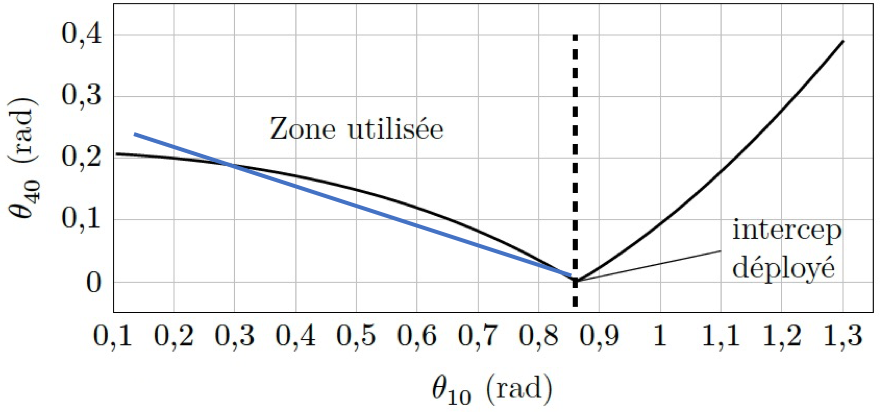
\includegraphics[width=.95\textwidth]{images/fig_03.png}
\end{center}
\end{minipage}



 
\end{UPSTIcorrige}

\subsection{Modélisation cinétique du mécanisme intercep, quantification de la dépense énergétique
liée au retrait compte tenu des exigences du désherbage mécanique}
\UPSTIobjectif{Ajouter, dimensionner et commander un actionneur électrique permettant d’assurer le mouvement de
retrait puis le déploiement de la lame.}


\subsubsection{Expression de l’énergie cinétique du mécanisme intercep}

\UPSTIobjectif{Exprimer l’énergie cinétique du mécanisme intercep dans un référentiel galiléen en fonction du seul
paramètre cinématique $\dot{\theta}_{40}$.}

\UPSTIquestion  Exprimer la projection du moment cinétique en $G_4$ du solide 4 dans son mouvement par rapport à 2
sur $\vect{z_0}=\vect{z_2}$, notée $\vectmc{G_4}{4}{2}\cdot\vect{z_2}$, puis exprimer l’énergie cinétique du solide 4 dans son mouvement par rapport à 2, $\ec{4}{2}$ en fonction de $I_{zz}$, $\dot{\theta}_{40}$, $M_4$ et $V_G = \left|\left| \vectv{G_4}{4}{2} \right|\right|$.

\begin{UPSTIcorrige}
\textbf{Expression du moment cinétique}

On a en $G_4$, centre d'inertie de la lame $\vectmc{G_4}{4}{2}\cdot \vect{z_2} = \left(\inertie{G_4}{\text{lame}}\vecto{4}{0}\right) \cdot\vect{z_2}$ 
$ = \matinertie{I_{xx}}{I_{yy}}{I_{zz}}{-I_{yx}}{-I_{xz}}{-I_{xy}}{G_4,\mathcal{B}_4} 
\begin{pmatrix} 0 \\ 0 \\ \dot{\theta}_{40} \end{pmatrix}_{\mathcal{B}_4} \cdot\vect{z_2}
$
$= \left(-I_{xz} \vect{x_4}-I_{yx} \vect{y_4}+I_{zz} \vect{z_4}\right)\dot{\theta}_{40} \cdot \vect{z_4}$
$= \dot{\theta}_{40}  I_{zz}$.

\textbf{Expression de l'énergie cinétique}
Par définition, $\ec{4}{2} = \dfrac{1}{2}\torseurci{4}{2} \otimes \torseurcin{V}{4}{2}$
$ = \dfrac{1}{2}\torseurl{\vectrc{4}{2}}{\vectmc{G_4}{4}{2}}{G_4} \otimes \torseurl{\vecto{4}{2}}{\vectv{G_4}{4}{2}}{G_4} $
$ = \dfrac{1}{2}\torseurl{M_4 \vectv{G_4}{4}{2}}{\vectmc{G_4}{4}{2}}{G_4} \otimes \torseurl{\dot{\theta}_{40}\vect{z_2}}{\vectv{G_4}{4}{2}}{G_4} $
$ = \dfrac{1}{2} \left(M_4 V_G^2 +\dot{\theta}_{40}^2  I_{zz} \right)$.

\end{UPSTIcorrige}



\UPSTIquestion  Exprimer le vecteur vitesse du point $G_4$ fixe dans 4 dans son mouvement par rapport à 2, noté $\vectv{G_4}{4}{2}$, sous sa forme la plus simple.

\begin{UPSTIcorrige}
Le point $O_1$ est fixe par rapport au solide 2 et le point $G_4$ est fixe par rapport au solide 4 on a donc,

$\vectv{G_4}{4}{2} = \dfrac{\dd }{\dd t} \left[\vect{O_1 G_4}\right]_{\mathcal{B}_2} $
$ = \dfrac{\dd  }{\dd t} \left[ -l_1 \vect{x_1} +  x_{G_4} \vect{x_4}+ y_{G_4} \vect{y_4}+ z_{G_4} \vect{z_4}\right]_{\mathcal{B}_2} $.

Par ailleurs, $\dfrac{\dd }{\dd t}\left[\vect{x_1}\right]_{\mathcal{B}_2}=\dot{\theta}_{10} \vect{y_1}$, 
$\dfrac{\dd }{\dd t}\left[\vect{x_4}\right]_{\mathcal{B}_2}=\dot{\theta}_{40} \vect{y_4}$, 
$\dfrac{\dd }{\dd t}\left[\vect{y_4}\right]_{\mathcal{B}_2}=-\dot{\theta}_{40}\vect{x_4}$ et
$\dfrac{\dd }{\dd t}\left[\vect{z_4}\right]_{\mathcal{B}_2}= \vect{0}$.

On a donc $\vectv{G_4}{4}{2} =-l_1\dot{\theta}_{10} \vect{y_1} +  x_{G_4} \dot{\theta}_{40} \vect{y_4}- y_{G_4} \dot{\theta}_{40} \vect{x_4}$.

\end{UPSTIcorrige}



\UPSTIquestion  En complément du programme de la figure 6, écrire une fonction Python \texttt{ktheta} qui prend en
paramètre les tableaux \texttt{theta40} et \texttt{theta10} et renvoie un tableau image de la fonction $k_{\theta}\left(\theta_{40}\right)$ telle que $\dot{\theta}_{10}=k_{\theta}\left( \theta_{40}\right)\dot{\theta}_{40}$.

\begin{UPSTIcorrige}

On a $
k_{\theta}=\dfrac{\dot{\theta}_{10}}{\dot{\theta}_{40}}=\dfrac{\dfrac{\dd \theta_{10}}{\dd t}}{\dfrac{\dd \theta_{40}}{\dd t}}
$.
On peut approximer $k_{\theta}$ par différence finie :
$
k_{\theta}\approx \dfrac{\dfrac{\Delta \theta_{10}}{\Delta t}}{\dfrac{\Delta \theta_{40}}{\Delta t}}\approx \dfrac{\Delta \theta_{10}}{\Delta \theta_{40}}
$.

\begin{lstlisting}
def ktheta (theta40,theta10):
    tktheta=[0]
    for i in range(1,len(theta40)):
        tktheta.append((theta40[i]-theta40[i-1])/(theta10[i]-theta10[i-1]))
    return tktheta 
\end{lstlisting}

\end{UPSTIcorrige}



\UPSTIquestion  Exprimer l'énergie cinétique du solide 4 dans son mouvement par rapport à 2, notée $\ec{4}{2}$, en fonction de $I_{zz}$, $\dot{\theta}_{40}$, $M_4$ et $\left(d\left(\theta_{40}\right)\right)^2$.

\begin{UPSTIcorrige}
On a vu que $ \ec{4}{2} = \dfrac{1}{2} \left(m_4 V_G^2 +\dot{\theta}_{40}^2  I_{zz} \right)$; donc 
$ \ec{4}{2} = \dfrac{1}{2} \left(M_4   \left(d\left( \theta_{40}\right) \right)^2 \dot{\theta}^2_{40} +\dot{\theta}_{40}^2  I_{zz} \right)$.

Au final, $ \ec{4}{2} = \dfrac{1}{2}  \dot{\theta}_{40}^2 \left(M_4   \left(d\left( \theta_{40}\right) \right)^2 +  I_{zz} \right)$.
\end{UPSTIcorrige}


\subsubsection{Implantation et choix de l’actionneur}

\UPSTIobjectif{À partir de l’équation de mouvement du mécanisme intercep, identifier les cas extrêmes et choisir un
actionneur.}



\UPSTIquestion  Exprimer sous forme littérale :
\begin{itemize}
\item la puissance des inter-efforts entre les solides 5 et 6 notée $\pint{5}{6}{}$ en fonction de $F_{\text{mot}}$ et $\dot{\lambda}$;
\item la puissance de l’action mécanique du sol sur 4 dans son mouvement par rapport à 2 notée $\pext{\text{sol}}{4}{2}$ en fonction de $F_{\text{sol}}$, $\dot{\theta_{10}}$, $\dot{\theta_{40}}$, $l_1$, $l_4$, $\theta_{41}$ et $\alpha_4$.
\end{itemize}

\begin{UPSTIcorrige}
\textbf{Puissance $\pint{5}{6}{}$}

Par définition, $\pint{5}{6}{} = \torseurstat{T}{5}{6}\otimes \torseurcin{V}{6}{5}$. On a 
$ \torseurstat{T}{5}{6} = \torseurl{F_{\text{mot}}\vect{x_5} + Y_{56}\vect{y_5}+ Z_{56}\vect{z_5}}{\vectm{V_2}{5}{6}}{V_2}$
et 
$\torseurcin{V}{6}{5} = 
\torseurl{\vect{0}}{
\dfrac{\dd }{\dd t}\left[\vect{V_1V_2}\right]_{\mathcal{B}_5}
}{V_2}=\torseurl{\vect{0}}{\dot{\lambda}\vect{x_5}}{V_2}$.
On a donc $\pint{5}{6}{} =F_{\text{mot}}\dot{\lambda}$. 

\textbf{Puissance $\pext{\text{sol}}{4}{2}$}

Par définition, on a $\pext{\text{sol}}{4}{2} = \torseurstat{T}{\text{sol}}{4} \otimes \torseurcin{V}{4}{2}$
$ = \torseurl{\vectf{\text{sol}}{4}}{\vectm{G_4}{\text{sol}}{4}}{G_4} \otimes \torseurl{\vecto{4}{2}}{\vectv{G_4}{4}{2}}{G_4}$

$ = \torseurl{-F_{\text{sol}}\vect{u_4}}{\vect{0} + \vect{G_4 B} \wedge -F_{\text{sol}}\vect{u_4}  }{G_4} \otimes \torseurl{\dot{\theta}_{40}\vect{z_0}}{\vectv{G_4}{4}{2}}{G_4} $ 
$ = \torseurl{-F_{\text{sol}}\vect{u_4}}{\left( -l_4 \vect{y_4} -  x_{G_4} \vect{x_4}- y_{G_4} \vect{y_4}- z_{G_4} \vect{z_4} \right)\wedge -F_{\text{sol}}\vect{u_4}  }{G_4} \otimes \torseurl{\dot{\theta}_{40}\vect{z_0}}{\vectv{G_4}{4}{2}}{G_4} $ 

$
=-F_{\text{sol}}\vect{u_4} \cdot \vectv{G_4}{4}{2} + \left(\left( -l_4 \vect{y_4} -  x_{G_4} \vect{x_4}- y_{G_4} \vect{y_4}- z_{G_4} \vect{z_4} \right)\wedge -F_{\text{sol}}\vect{u_4}  \right)\cdot \dot{\theta}_{40}\vect{z_0}
$. 

En utilisant les propriétés du produit mixte, on a 
$
\pext{\text{sol}}{4}{2} =-F_{\text{sol}}\vect{u_4} \cdot \vectv{G_4}{4}{2} + \left(\left( -l_4 \vect{y_4} -  x_{G_4} \vect{x_4}- y_{G_4} \vect{y_4}\right)\wedge -F_{\text{sol}}\vect{u_4}  \right)\cdot \dot{\theta}_{40}\vect{z_0}
$.

Par suite $
\pext{\text{sol}}{4}{2} =-F_{\text{sol}}\vect{u_4} \cdot \left( -l_1\dot{\theta}_{10} \vect{y_1} +  x_{G_4} \dot{\theta}_{40} \vect{y_4}- y_{G_4} \dot{\theta}_{40} \vect{x_4}\right) + \left(\left( l_4 \vect{y_4} +  x_{G_4} \vect{x_4}+ y_{G_4} \vect{y_4}\right)\wedge \vect{u_4}  \right)\cdot F_{\text{sol}} \dot{\theta}_{40}\vect{z_0}$

$=-F_{\text{sol}} \left( -l_1\dot{\theta}_{10}\cos\left( -\alpha_4 - \theta_{40} +\dfrac{\pi}{2} + \theta_{10}\right) +  x_{G_4} \dot{\theta}_{40}\sin \alpha_4- y_{G_4} \dot{\theta}_{40}\cos\alpha_4\right)  + \left( \sin \alpha_4 x_{G_4} - \cos \alpha_4 \left( l_4 + y_{G_4}\right) \right)\cdot F_{\text{sol}} \dot{\theta}_{40}$
$=-F_{\text{sol}} l_1\dot{\theta}_{10}\sin\left(  \theta_{10}-\alpha_4 - \theta_{40}\right)     - l_4  F_{\text{sol}} \dot{\theta}_{40} \cos \alpha_4 $. 

En réalisant une fermeture angulaire, $\theta_{41} = \theta_{40} -\theta_{10}$ et
$\pext{\text{sol}}{4}{2}=F_{\text{sol}} l_1\dot{\theta}_{10}\sin\left(  \theta_{41}+\alpha_4 \right)     - l_4  F_{\text{sol}} \dot{\theta}_{40} \cos \alpha_4 $. 



\end{UPSTIcorrige}


\UPSTIquestion Exprimer la masse équivalente $M_{eq}$ en fonction de $I_{zz}$, $M_4$, $d\left(\theta_{40}\right)$ et $k\left(\theta_{40}\right)$ telle que l’énergie cinétique de l’ensemble \{1+4+5+6\} dans son mouvement par rapport à 2 soit égale à $\dfrac{1}{2}M_{eq} \dot{\lambda}^2$.

\begin{UPSTIcorrige}
Les masses et les inerties des solides 1, 5 et 6 étant négligeables, $  \ec{1+4+5+6}{2}$ $=\ec{4}{2}$ $= \dfrac{1}{2}  \dot{\theta}_{40}^2 \left(M_4   \left(d\left( \theta_{40}\right) \right)^2 +  I_{zz} \right)$ (Question 14). 

On a alors  $\ec{4}{2}= \dfrac{1}{2} \left( k_{\lambda} \left(\theta_{40}\right)\right) ^2\dot{\lambda}^2 \left(M_4   \left(d\left( \theta_{40}\right) \right)^2 +  I_{zz} \right)$.

On a donc $M_{eq}=  \left( k_{\lambda} \left(\theta_{40}\right)\right) ^2 \left(M_4   \left(d\left( \theta_{40}\right) \right)^2 +  I_{zz} \right)$.
\end{UPSTIcorrige}



\UPSTIquestion  En indiquant le système isolé et le théorème utilisé, exprimer littéralement $F_{\text{mot}}$ en fonction de $\ddot{\lambda}$, $M_{\text{eq}}$, $F_{\text{sol}}$ et $k_p\left(\theta_{40}\right)$. Effectuer l’application numérique dans le pire des cas pour l’actionneur ($F_{\text{sol}} = F_{d \text{MAX}}=\SI{5}{kN}$),
indiquer la position choisie pour la valeur de $\theta_{40}$ (figure 9) et l’état (1 ou 2 de la figure C) le plus critique.

\begin{UPSTIcorrige}

\textbf{Expression de $F_{\text{mot}}$}

On isole  \{1+4+5+6\} et on applique le théorème de l'énergie cinétique. 

Bilan des puissances extérieures : 
\begin{itemize}
\item puissance de la pesanteur nulle (mouvement dans un plan orthogonal à $\vect{g}$);
\item puissance de l'action du sol sur la lame 
$\pext{\text{sol}}{4}{2}=-F_{\text{sol}}k_p\left(\theta_{40}\right)\dot{\lambda}$.
\end{itemize}

Bilan des puissances intérieures :
\begin{itemize}
\item les liaisons sont parfaites. Elles ne dissipent donc pas de puissance;
\item puissance $\pint{5}{6}{}=F_{\text{mot}}\dot{\lambda}$.
\end{itemize}




Calcul de l'énergie cinétique : $\ec{1+4+5+6}{2} =\ec{4}{2} = \dfrac{1}{2}M_{\text{eq}}\dot{\lambda}$.

On applique le théorème de l'énergie cinétique, et on obtient : 
$\dfrac{\dd \ec{4}{2}}{\dd t}= \pint{5}{6}{}+\pext{\text{sol}}{4}{2}$.
$\Leftrightarrow 
M_{eq} \dot{\lambda}\ddot{\lambda}=  F_{\text{mot}}\dot{\lambda}
-F_{\text{sol}}k_p\left(\theta_{40}\right)\dot{\lambda}$
$\Leftrightarrow 
M_{eq} \ddot{\lambda}=  F_{\text{mot}}
-F_{\text{sol}}k_p\left(\theta_{40}\right)$ ($\dot{\lambda}\neq 0$).

 Au final,   $F_{\text{mot}}=M_{eq} \ddot{\lambda} + F_{\text{sol}}k_p\left(\theta_{40}\right)$.

\textbf{Application numérique}



Dans le pire des cas, $F_{\text{sol}} = F_{d \text{MAX}}=\SI{5}{kN}$, $k_p\left(\theta_{40}\right) \simeq 3$ et $M_{eq}=\SI{300}{kg}$ pour $\theta_{40}=\SI{0,21}{rad}$.

\begin{itemize}
\item Dans l'état 1, asservissement du mouvement de retrait : $\ddot{\lambda}=12 m\cdot s^{-2}$. On a donc  $F_{\text{mot}}=300 \times  12 + 5000\times 3 = \SI{18 600}{N}$.
\item Dans l'état 2, mouvement de déploiement en BO de vitesse : $\ddot{\lambda}=-10 m\cdot s^{-2}$. On a donc  $F_{\text{mot}}=300 \times  -10 + 5000\times 3 = \SI{12 000}{N}$.
\end{itemize}

L'état 1 est le plus critique.


\end{UPSTIcorrige}





\UPSTIquestion  Conclure sur le choix de l'actionneur en proposant une des références du tableau 2.

\begin{UPSTIcorrige}
En se basant sur l'effort maximal, le vérin 4 convient (avec une marge importante).  Dans le pire des cas, l'accélération de \SI{12}{m.s^{-2}} dure \SI{0,1}{s}. La vitesse atteinte est donc de \SI{1,2}{m.s^{-1}}; en se basant sur la vitesse maximale, le vérin 4 convient donc. 

Tous les vérins ont la même course. Sous réserve que la course nécessaire au vérin soit inférieure à \SI{400}{mm}, on choisit donc le vérin 4. 
\end{UPSTIcorrige}

\subsection{Commande de l’actionneur}
\UPSTIobjectif{ Valider le pilotage séquentiel de l’actionneur et choisir un correcteur pour la boucle de vitesse vis-à-vis des exigences du désherbage mécanique.}

\UPSTIquestion  À partir du diagramme d’état de la figure C, compléter les chronogrammes de la figure D du document réponse. Justifier la pertinence de la prise en compte des deux évènements «~after(\SI{0,25}{s})~» et «~after(\SI{0,1}{s})~» vis-à-vis de l’exigence 1.2 sur la protection des ceps en indiquant les problèmes qu’ils pallient. Justifier également que le choix d’une chaine de transmission réversible permet d’assurer le déverrouillage de l’outil.

\begin{UPSTIcorrige}
\begin{center}
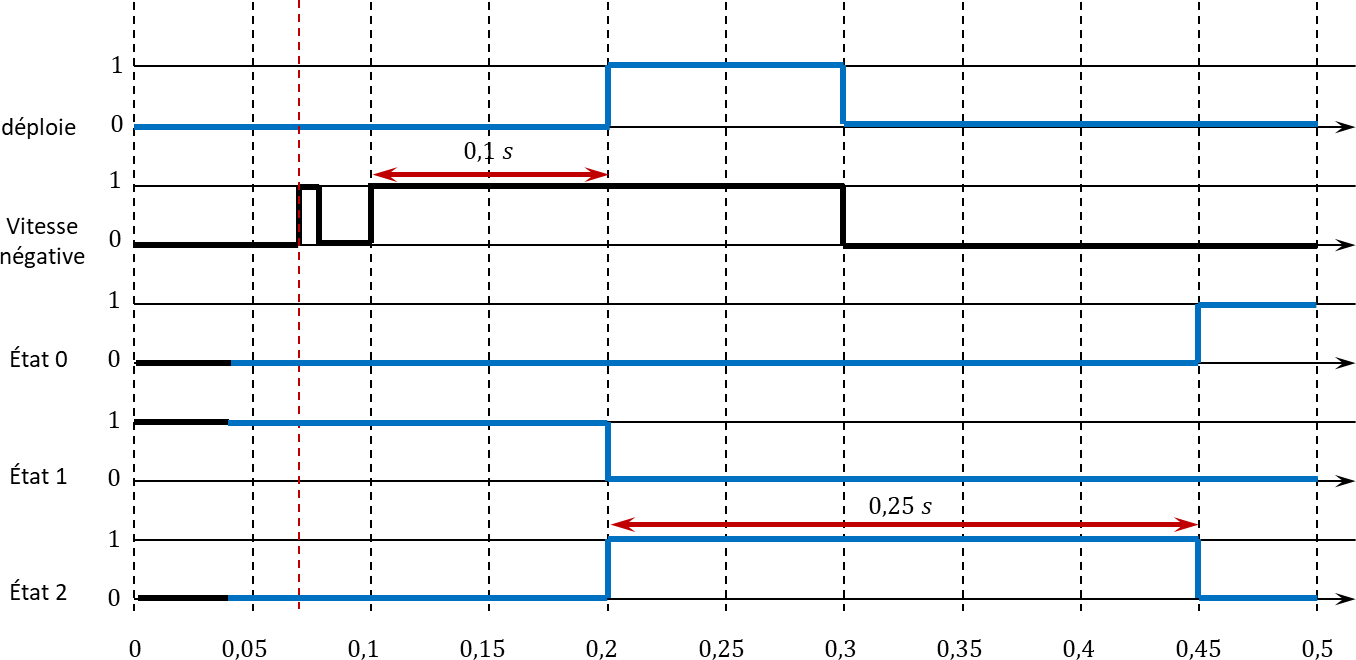
\includegraphics[width=.8\textwidth]{images/fig_04.png}
\end{center}

À 0,3 s, il semble que deux évènements se produisent en même temps et ils correspondent à deux transition de l'état "détection du retour de la barre palpeuse" : \textbf{after(0,1s)} et \textbf{!vitesse négative}.

\textbf{Prise en compte des événements after}

L'exigence 1.2 concerne la protection des ceps. Elles nécessite :
\begin{itemize}
\item de déverrouiller les outils interceps si l'effort résistant à l'avancement dépasse un seuil  $F_d$ réglable entre $\SI{0,1}{kN}$ et $\SI{5}{kN}$ ;
\item d'éviter les ceps en jouant sur le déploiement des lames.
\end{itemize}

Les deux évènements «~after(\SI{0,25}{s})~» et «~after(\SI{0,1}{s})~» permettant alors de répondre à cette exigence : 
\begin{itemize}
\item «~after(\SI{0,1}{s})~» permet d'assigner la variable logique déploie à 1 si la vitesse reste négative plus de \SI{0,1}{s} pour s'assurer qu'il y a bien un obstacle et éviter des fausses alertes;
\item «~after(\SI{0,25}{s})~» permet de ne pas rester trop longtemps en mouvement de déploiement en BO (état 2) si la vitesse reste négative (suspicion de détection de cep). Si la vitesse redevient positive l’événement \textbf{!vitesse negative} se produit et on repasse en asservissement en vitesse sinon on bascule dans l'état déverrouillage.
\end{itemize}

\textbf{Choix de la chaine de transmission}


La chaine de transmission est réversible car le mode d'asservissement étant en vitesse et celle-ci pouvant être négative ou négative il faut pouvoir générer une commande bilatérale.


\end{UPSTIcorrige}





\UPSTIquestion  Proposer, en justifiant la réponse, la forme du correcteur à choisir parmi $K_P$, $\dfrac{1}{Ti_p}$, $K_i \dfrac{1+T_i p}{T_i p}$ et $K_d \dfrac{1+T_d p}{1+\alpha T_d p}$ afin qu’un simple réglage manuel de la position de la barre palpeuse permette de satisfaire l’exigence 1.2.2 (il n’est pas demandé de régler les paramètres du correcteur choisi).

\begin{UPSTIcorrige}
\begin{itemize}
\item On souhaite une erreur de trainage vis-à-vis d'une consigne en vitesse nulle, il faut donc que la classe de la FTBO de la boucle en vitesse soit au moins égale à 2. Il faut donc au moins une intégration supplémentaire dans la boucle ouverte. On peut donc choisir : $C(p)=\dfrac{1}{T_ip}$ ou $C(p)=K_i\dfrac{1+T_ip}{T_ip}$.
\item Avec ces deux types de correcteurs (intégral ou proportionnel intégral), on met en place une classe égale à 1 en amont de la perturbation, ainsi la précision de l'asservissement est insensible à une perturbation de type échelon ($-F_{\text{sol}}k_{p\text{MAX}}$) ou supposée constante.
\item Ces deux types de correcteurs permettent de régler la bande passage de la boucle ouverte soit en jouant sur $T_i$ pour le premier, soit sur $K_i$ et/ou $T_i$ pour le second. 
\item Un critère de stabilité non défini dans le sujet permettrait de choisir le second correcteur car il permettrait d'apporter un déphasage nul au delà d'une certaine pulsation et de permettre ainsi de régler correctement les marges de stabilité.
\end{itemize}
\end{UPSTIcorrige}



\section{Synthèse}


\UPSTIquestion  À partir des courbes de la figure 11, issues de la simulation numérique effectuée :
\begin{itemize}
\item expliquer ce qui se passe physiquement au niveau du contact roues–sol au cours du temps ;
\item analyser l’allure et l’amplitude des évolutions de $\delta_F$ et $\delta_R$ . Justifier si ce résultat est conforme à celui qui est attendu de la part du robot.
\end{itemize}

\begin{UPSTIcorrige}
\begin{itemize}
\item La trajectoire à réaliser est une ligne droite suivant la direction $\vect{x}$.
\item Après \SI{3}{m}, les roues arrières tournent de \SI{0,5}{\degres} dans le sens horaire (vers la droite). Les roues avant commencent à tourner dans le sens trigonométrique (vers la gauche).  On a alors $\beta_F \simeq \delta_F$ et $\beta_R \simeq \delta_R$. On peut donc supposer que les roues avant adhèrent alors que les roues arrières glissent. Cette situation créent un écart du véhicule dans la direction $-\vect{y}$.
\item Après \SI{6}{m}, toutes les roues tournent dans le sens positif. Cela permet au véhicule de revenir sur sa trajectoire et cela au bout de \SI{20}{m}. 
\item Il est alors nécessaire de remettre les roues droites. Au début de cette phase, les roues arrières glissent légèrement, puis toutes les roues tournent dans le sens horaires afin de revenir en position droite.
\end{itemize}

Durant la trajectoire l'amplitude de $\delta_F$ et $\delta_R$ est inférieure à 6\degres, ce qui est conforme avec l'hypothèse d'angles faibles. De plus,  l'hypothèse $\delta_F'\simeq \delta_R'$ (page 7 du sujet) est vérifiée. 
\end{UPSTIcorrige}



\UPSTIquestion  À partir des courbes issues de la simulation numérique effectuée (figures 11 et 12) :
\begin{itemize}
\item vérifier si les hypothèses émises (relatives à la valeur des différents angles, ainsi qu’à leur variation le long
de la trajectoire à suivre), afin de déterminer des lois simples pour obtenir les valeurs d’angle de consigne
d’orientation des roues avant et arrière $\delta_F^*$ et $\delta_R^*$, sont validées. Justifier quantitativement la réponse;
\item conclure quant à la validité des lois de génération de consigne d’orientation des roues proposées et des valeurs
des paramètres $K_{dF}$, $K_{pF}$ et $K_{dR}$ retenues, vis-à-vis du cahier des charges en terme de précision de guidage du robot enjambeur ;
\item conclure quant à l’aptitude du robot Bakus à pouvoir désherber mécaniquement sous un rang de vigne à
l’aide d’un outil intercep, en tenant compte de l’exigence de guidage.
\end{itemize}

\begin{UPSTIcorrige}
\begin{itemize}
\item Lorsque les roues arrières glissent, $y_{G_2}$ devient négatif donc l'engin dévie sur la droite et $\theta$ est positif donc son orientation est dans le sens trigonométrique.
\item Au bout de $\SI{25}{s}$, $\theta$ et $y_{G_2}$ sont nuls donc le véhicule est bien dirigés selon $\vect{x}_0$.
\item La stratégie de commande de l'engin semble donc fonctionner. Le centre de gravité reste à moins de $\SI{4,1}{mm}$ de la position médiane et avec $\vert\theta\vert<\SI{0,1}{\degres}$ on obtient en position extrême $y_R=L\tan \theta=$. Il faudrait la valeur de $L$ pour conclure.
\item La précision de guidage du robot enjambeur semble satisfaisante puisque $\vert y_{G_2}\vert <\SI{4,1}{mm}$ alors que le cahier des charges avec l'exigence 1.1.3 demandait $\vert y_{G_2}\vert<\SI{2}{cm}$ ainsi les valeurs des paramètres $K_{dF}$, $K_{pF}$ et $K_{dR}$ retenues semblent correctes.
\item Ainsi le robot Bakus semble tout à fait capable de désherber mécaniquement sous un rang de vigne à partir des exigences proposées dans le sujet.
\end{itemize}
\end{UPSTIcorrige}




%\UPSTIquestion  QUESTION
%\begin{UPSTIcorrige}
%TODO
%\end{UPSTIcorrige}
%
%% -------------------------- 
%% Question
%% -------------------------- 
%\UPSTIquestion Intitule de la question
%
%$\vecto{1}{2}$, $\vectv{A}{1}{2}$
%
%$\vectf{1}{2}$, $\vectm{A}{1}{2}$
%
%$\vectrc{1}{2}$, $\vectmc{A}{1}{2}$
%
%$\vectrd{1}{2}$, $\vectmd{A}{1}{2}$
%
%$\vectg{A}{1}{2}$
%
%$\ec{A}{B}$
%
%$\pint{A}{B}{C}$
%
%$\pext{A}{B}{C}$
%
%\begin{UPSTIcorrige}
%Corrigé de la question... Lorem ipsum dolor sit amet consectetuer Morbi Nunc lacus vitae gravida. Morbi ridiculus non interdum nibh consequat malesuada natoque tincidunt sed neque. Interdum felis quis ut id hendrerit semper natoque nisl Cum ipsum.
%\end{UPSTIcorrige}
%% -------------------------- 
%
%% -------------------------- 
%% Question sans intitulé... juste le numéro (déconseillé)
%% -------------------------- 
%\UPSTIquestion
%
%\begin{UPSTIcorrige}
%Ici on a une question sans intitulé....
%
%Lorem ipsum dolor sit amet consectetuer Morbi Nunc lacus vitae gravida. Morbi ridiculus non interdum nibh consequat malesuada natoque tincidunt sed neque. Interdum felis quis ut id hendrerit semper natoque nisl Cum ipsum. 
%\end{UPSTIcorrige}
%% -------------------------- 
%
%%---------------------------------%
%% FIN du contenu
%%---------------------------------%

\end{document}
